\documentclass{article}
\usepackage[top=2cm, bottom=2cm, left=2.2cm, right=2.5cm]{geometry}
\usepackage{amsmath,amsfonts,amssymb}
\usepackage{enumerate}% http://ctan.org/pkg/enumerate

\usepackage[]{pdfcomment}
%As recommended by matlab2tikz
\usepackage{pgfplots}
\usepackage{tikz}
\usepackage{nicematrix}
\usepackage{calc}
\usepackage{pgfplotstable}
\usepackage{booktabs}
\usepackage{csvsimple}
\usepackage{etoolbox}
\usepackage[style=alphabetic]{biblatex}
\usepackage{amsthm}
\bibliography{refs.bib}
%% the following commands are needed for some matlab2tikz features
\usetikzlibrary{plotmarks}
\usetikzlibrary{arrows.meta}
\usepgfplotslibrary{patchplots}
\usepackage{grffile}
%% you may also want the following commands
\pgfplotsset{plot coordinates/math parser=false}
%\newlength\figureheight
%\newlength\figurewidth
\usepackage{hyperref}
\usepackage{placeins,nicefrac}
\usepackage{xstring}
\usepackage[]{pgfkeys}
\usepackage{xfrac}
\usepackage[newfloat]{minted}
\usetikzlibrary{external}
\usetikzlibrary{calc,math}
\tikzexternalize[prefix=extern/]
\usepgfplotslibrary{groupplots}
\usepgfplotslibrary{colormaps}
\usetikzlibrary{decorations.markings,patterns,patterns.meta,pgfplots.fillbetween}

\usepackage[ruled,vlined,linesnumbered,algo2e]{algorithm2e}
\usepackage{wrapfig}
\usepackage{subcaption}
\newenvironment{code}{\captionsetup{type=listing}}{}
\SetupFloatingEnvironment{listing}{name=Source Code}
\graphicspath{../plots/}

\usepackage{wasysym}
\usepackage{animate}

%\usepackage{expl3}
%\ExplSyntaxOn
%\cs_set_eq:NN \fpeval \fp_eval:n
%\ExplSyntaxOff

\usetikzlibrary{fpu}
\graphicspath{{../figs/}}
\newcommand{\figurescale}{1.0}

%\usepackage{titlesec}
%\titleformat{\subsection}{\normalfont\large\bfseries}{Task \thesubsection}{1em}{}
%\titleformat{\section}{\normalfont\Large\bfseries}{Assignment \thesection}{1em}{}
%\titleformat{\subsubsection}{\normalfont\bfseries}{Question \thesubsubsection}{1em}{}
\newcommand\mycommfont[1]{\ttfamily\textcolor{blue}{#1}}
\SetCommentSty{mycommfont}

\newcommand{\stilltodo}[1]{{\color{red} UNFINISHED #1}}

\makeatletter
\newcommand{\trp}{%
	{\mathpalette\@transpose{}}%
}
\newcommand*{\@transpose}[2]{%
	% #1: math style
	% #2: unused
	\raisebox{\depth}{$\m@th#1\intercal$}%
}

\makeatother
\newcommand{\diff}{\mathrm{d}}
\author{Andr\'as Schifferer, r0915705}
\title{Numerical Linear Algebra [H03G1A]\\{\LARGE HW1}\\{\large Practical L\'anczos method}}
\date{\today} 

\pgfplotsset{plot coordinates/math parser=false}

\makeatletter
\providecommand{\leftsquigarrow}{%
	\mathrel{\mathpalette\reflect@squig\relax}%
}
\newcommand{\reflect@squig}[2]{%
	\reflectbox{$\m@th#1\rightsquigarrow$}%
}
\makeatother


\newtheorem{lemma}{Lemma}
\newtheorem{theorem}{Theorem}


\begin{document}
	\maketitle
	%The assignment is not yet finished unfortunately.
	\tableofcontents
	
	
	
	\newpage
	\section{Semi-Orthogonality and strategic reorthogonalization}
	\textit{Note that throughout the first part of the assignment if an algorithm is performed on an unspecified matrix, then the subjected matrix should be understood to be the one provided for the assignment as \texttt{Test.mtx}.
	}
	
	The Lánczos algorithm can be used to construct a Hessenberg decomposition of a matrix plus a rank 1 term. If we restrict the matrix inputs to real symmetric matrices, then the symmetry requirement will force the apprximately similar Hessenberg matrix to be symmetric as well, which results necessarily in a tridiagonal matrix.
	\begin{algorithm2e}[ht]
		
		\SetKwInOut{Input}{input}
		\SetKwInOut{Output}{output}
		\SetKw{Init}{init}{}{}
		\SetAlgoLined
		\Input{Linear, symmetric real operator $A$ on $\mathbb{R}$}
		\Output{Approximately orthogonally similar tridiagonal $T\sim A$, given by diagonals $\mathbf{\alpha},\mathbf{\beta}$}
		\Init{choose starting vector $\mathbf{r}_0$,$\beta_0:=\|\mathbf{r}_0\|$, $\mathbf{q}_0=0$}\\
		\For{$j=1,2,...$}{
			$\mathbf{q}_j:=\mathbf{r}_{j-1}/\beta_{j-1}$\\
			$\mathbf{v}_j=A\mathbf{q}_j-\beta_{j-1}\mathbf{q}_{j-1}$\\
			$\alpha_j=\mathbf{v}_j^{\ast}\mathbf{q}_j$\\
			$\mathbf{r}_j=\mathbf{v}_j-\alpha_j\mathbf{q}_j$\\
			$\beta_j=\|\mathbf{r}_j\|$\\
		}
		\caption{Lanczos in exact arithmetic (Lanczos0)}\label{alg:Lanczos0}
	\end{algorithm2e}\\
	
	The matrix $T$ then has the form 
	$$T=\begin{pmatrix}
		\alpha_1&\beta_1&0&\cdots&0\\
		\beta_1&\alpha_2&\beta_2&&0\\
		\vdots&\ddots&\ddots&\ddots&\vdots\\
		0&&\beta_{j-2}&\alpha_{j-1}&\beta_{j-1}\\
		0&\cdots&0&\beta_{j-1}&\alpha_{j}\\
	\end{pmatrix}$$
	One step in the main loop of \autoref{alg:Lanczos0} is called a Lanczos step, and is usually written as
	\begin{equation}\label{eq:LanczosStep}
		\beta_j\mathbf{q}_{j+1}=A\mathbf{q}_j-\alpha_j\mathbf{q}_j-\beta_{j-1}\mathbf{q}_{j-1}.
	\end{equation}
%\part{title}	\inputminted[firstline=2, lastline=5]{matab}{../NLAHW1_Lanczos/test.m}
	
	We know that, with $Q_{j}:=[\mathbf{q}_1,\ldots,\mathbf{q}_j]$, we have the relation
	\begin{equation}\label{eq:matLanczos}
		AQ_{j}=Q_jT_j+\beta_{j}\mathbf{q}_{j+1}\mathbf{e}^{\ast}.
	\end{equation}
	In exact arithmetic the above is a great procedure for tridiagonalization. Numerically this is
	not the case unfortunately, as the orthogonality of $Q$ gets diminished by numerical errors.
	
	\subsection{Lanczos0: 'theoretical' Lanczos' problems}
	
	The theoretical Lanczos algorithm (hereby reffered to as Lanczos0) will lose stability after only a small number of iterations, as examplified in \autoref{fig:lanczos0_W}
	\begin{figure}
		\centering
		\resizebox{\textwidth}{!}{
		\input{../plots/lanczos0_W.tex}}
		\caption{Loss of orthogonality in Lanczos 0}\label{fig:lanczos0_W}
	\end{figure}
	
	 The figure uses the "orthogonality matrix" $W_j$, which is hereby defined as
	\begin{equation}
		W_j = Q_j^\ast Q_j,
	\end{equation}
	where the higher the values of this matrix are, the less orthogonal the two correspondin vectors are.
	We can see that in \autoref{fig:lanczos0_W} orthogonality is maintained in comparison to the previous vectors roughly for the last 20 vectors, and after the same number of iterations for some vector pairs orthogonality is completely and irreovcably lost.
	
	This can be further corrobarated by the convergence of the Ritz values as seen in \autoref{fig:lanczos0_W_ritz}.
	Note that the test matrix (provided in \texttt{Test.mtx}) only has real eigenvalues more than or equal to one. We can see that in 
	comparison with the better performing \texttt{Lanczos1} algorithm (to be discussed later) where the Ritz values seem to be doing a good job approximating the spectrum of eigenvalues (in \autoref{fig:lanczos1_W_ritz}). In contrast Lanczos0 has trouble fully covering the eigenvalues in the Test matrix. Even at higher iteration numbers (i.e. a larger number of Ritz values) sometimes a spurious Ritz value appears, for example between the two largest eigenvalues at $j=39$. This might be explained by the last vector having a too high component parallel to the eigenvector corresponding to a larger eigenvalue. Therefore this might change the eigenvalues of $T_k$, which results in a bad quality approximation of the spectrum.
	
	
	
	\subsection{Lanczos1: 'practical' Lanczos}
	% It is not practical because calculating Q*Q is a lot of effort
	In order to better preserve the orthogonality of all the vectors, periodic checks of the $W_j$ matrix would be desired coupled with full reorthogonalization. By the latter we mean that every component of other basis vectors is removed from the candidate $q_{j+1}$ as seen in \autoref{alg:reorthogonalization}, where the key step is
	\begin{equation}
		\textbf{r} \gets \textbf{r} - Q_{k-1} Q_{k-1}^\ast \textbf{r}.
	\end{equation}
	\begin{algorithm2e}[h!]
	\SetAlgoNlRelativeSize{-1}
	\caption{Reorthogonalization against all previous $\textbf{q}_i$}\label{alg:reorthogonalization}
	\KwIn{$Q_k$: Matrix with quasi-orthonormal columns}
	\KwIn{$\textbf{r}$: Vector to be reorthogonalized}
	\KwOut{$\textbf{r}_{\text{new}}$: Reorthogonalized vector}
	
	$\textbf{r} \gets \textbf{r} - Q_{k-1} Q_{k-1}^\ast \textbf{r}$\\
	$\alpha_{\text{loc}} \gets \textbf{q}_k^\ast \cdot r$\\
	$\textbf{r}_{\text{new}} \gets \textbf{r} - \alpha_{\text{loc}}  \textbf{q}_k$\\
\end{algorithm2e}
	
	To detect the lost of orthogonality we require that the offdiagonal elements of $W_j$ satisfy some condition, namely that they would not exceed some $\delta$ value so ast to
	\begin{equation}\label{eq:delta-orth-lim}
		w_{j,\infty}:=\|W_j-I_j\|_{\mathrm{max}} < \delta
	\end{equation}
 If $\delta = \sqrt{\frac{\epsilon}{j}}$, then the semi-orthogonality of $Q_j$ will be preserved, meaning that $w_{j, \infty} = \mathcal{O}\left(\sqrt{\epsilon}\right)$. 	\autoref{theore:quasi-orth} ensures that this will suffice to contain the errors of the method.
	
	\begin{theorem}\label{theore:quasi-orth}
		With notation from before, let $P_j$ denote the orthogonal basis for $\text{span}(Q_j)$.
		If $w_{j,\infty}<\sqrt{\frac{\epsilon}{j}}$ then
		$$\|P_j^{\ast}AP_j-T_j\|_{max}=\mathcal{O}(\epsilon\|A\|).$$ 
	\end{theorem}
	
	\begin{algorithm2e}[ht]
		
		\SetKwInOut{Input}{input}
		\SetKwInOut{Output}{output}
		\SetKw{Init}{init}{}{}
		\SetAlgoLined
		\Input{Linear, symmetric real operator $A$ on $\mathbb{R}$}
		\Output{Approximately orthogonally similar tridiagonal $T\sim A$, given by diagonals $\mathbf{\alpha},\mathbf{\beta}$}
		\Init{choose starting vector $\mathbf{r}_0$,$\beta_0:=\|\mathbf{r}_0\|$, $\mathbf{q}_0=0$, $W_0=\begin{bmatrix} 0 \end{bmatrix}$, \texttt{reorth\_next}=0, $\delta= \sqrt{\frac{\epsilon}{j}}$}\\
		\For{$j=1,2,...$}{
			$\mathbf{q}_j:=\mathbf{r}_{j-1}/\beta_{j-1}$\\
			$\mathbf{v}_j=A\mathbf{q}_j-\beta_{j-1}\mathbf{q}_{j-1}$\\
			$\alpha_j=\mathbf{v}_j^{\ast}\mathbf{q}_j$\\
			$\mathbf{r}_j=\mathbf{v}_j-\alpha_j\mathbf{q}_j$\\
			$\beta_j=\|\mathbf{r}_j\|$\\
			\tcc{   Is reorthogonalization needed?}
			\If{$j<k_{\text{max}}-1$ \textbf{and} $j>1$}{
				$W_{j} \gets Q_j^\ast Q_j$\tcp{Calculating $W_j$ via expensive matrix product}\label{line:Wj-by-matmul}
				$\omega_{j,\infty} \leftarrow  \lVert W_j-I_j \rVert_{\mathrm{max}}$\\
				\If{$\omega_{j,\infty} > \delta$}{
					\tcp{Reorthogonalization needed}
					\texttt{reorth\_next} $\gets$ 2\tcp{Reorthogonalize the next two vectors}\label{line:reorth-next}
					
				}
			}
			\tcc{   Reorthognalize if needed}
			\If{$\texttt{reorth\_next}>0$}{
				$\mathbf{r}_j, \beta_j \gets \text{reorthogonalization}(Q_k(:, 1:j), \mathbf{r}_j, \beta_j)$ \tcp{Reorthogonalize using \autoref{alg:reorthogonalization}}
				$W_j(1:end-1) \leftarrow \epsilon z_3$ \tcp{Reroll off-diagonal values}
				\texttt{reorth\_next} $\gets$ \texttt{reorth\_next}-1
			}
		}
		\caption{Lanczos1 with impractically detected full reorthogonalization}\label{alg:Lanczos1}
	\end{algorithm2e}
	
	The implementation of Lanczos1 can be seen in \autoref{alg:Lanczos1}, and has also been implemented in \texttt{Matlab}. An important pratical aspect to note is that while it would be enough to just reorthogonalize one of the vectors at each trigger of the condition, in practice though this leads to a more inefficient algoithm. The reason behind this is that as we can see in \autoref{eq:LanczosStep} (the Lanczos step), any new vector relies on the previous two. Therefore even if we reorthogonalize one of them, the one before could still allow to carry over and spread the numerical errors. To circumvent this we can just reorthogonalize two iterations in a row, which cuts of the spread of the floating point errors to the new vectors. This is why on \autoref{line:reorth-next} \texttt{reorth\_next} is set to 2 (this and following is reorthogonalized). 
	
	The numerical results of the algorithm shows good orthogonality preservation in \autoref{fig:lanczos1_W} as well as good convergence of the Ritz values in \autoref{fig:lanczos1_W_ritz}. Here the convergence of the latter is much more stable, once a good estimate has been found somewhere that won't wiggle around. 
	
	However, despite our best efforst, Lanczos1 loses a lot of the time efficiency of Lanczos0. This slowness is mainly caused by \autoref{line:Wj-by-matmul}, where the matrix multiplication can be in general of order $\mathcal{O}(n^3)$, and is performed each iteration. \autoref{ssec:lanczos2} will try to remedy this problem, by introducing a celever heuristic for estimating $\omega_{j,\infty}$.
	\begin{figure}
		\centering
		\resizebox{\textwidth}{!}{
			\input{../plots/lanczos1_W.tex}}
		\caption{Loss of orthogonality in Lanczos 1. Note that $w_{k,\infty}$ is always shown, as the one used in testing for reorthogonalization (i.e. the projected one in the next step)}\label{fig:lanczos1_W}
	\end{figure}
	
	\begin{figure}
	\centering
	\resizebox{0.95\textwidth}{!}{
		\includegraphics[trim=0 180 0 250 clip]{../plots/lanczos0_ritz.pdf}}
	\caption{Lanczos0: The eigenvalues of the test matrix ($\lambda_i$'s histogram) and the Ritz values at the $j^{\mathrm{th}}$ iteration ($\mu_i$, denoted by ${\color{red} \times}$ )}\label{fig:lanczos0_W_ritz}
	\end{figure}
	
	\begin{figure}
	\centering
	\resizebox{0.95\textwidth}{!}{
		\includegraphics[trim=0 170 0 180,clip]{../plots/lanczos1_ritz.pdf}}
	\caption{Lanczos1: The eigenvalues of the test matrix ($\lambda_i$'s histogram) and the Ritz values at the $j^{\mathrm{th}}$ iteration ($\mu_i$, denoted by ${\color{red} \times}$ )}\label{fig:lanczos1_W_ritz}
	\end{figure}
	
	\FloatBarrier
	
	\subsection{Lanczos2: heuristic for loss of orthogonality}\label{ssec:lanczos2}
	
	Calculating $W = Q^\ast Q$ was the most costly part of the Lanczos1 algorithm, especially since this step needs to be done at each iteration, to determine whether a correction is needed or not in the first place. Loss of orthogonality could be predicted using a parallel system for iteratively constructing $\tilde{W}$, which could serve as a proxy to gauge when loss of orthogonality is to be expected. Our main assumption going forward will be that floating point errors have comaprable behaviour to that of Gaussian noise.
	
	Ideally in exact arithmetic $W_j = \mathbb{I}_{j\times j}$ (identity) would hold. However if at each iteration, i.e. the calculation of the new $\textbf{q}_j$, we could have access to the exact arithmetic error (which is assumed to be random and therefore inaccessible), we could predict the evolution of the non-ideal $W_j$. First let's look at the Lanczos step in \autoref{eq:LanczosStep}. By adding the floating point error $\textbf{f}_j$
	the equation becomes
	\begin{equation}\label{eq:LanczosStep-f}
		\beta_j\mathbf{q}_{j+1}=A\mathbf{q}_j-\alpha_j\mathbf{q}_j-\beta_{j-1}\mathbf{q}_{j-1} - \textbf{f}_j.
	\end{equation}
	This can be transformed in a similar fashion as before into 
	\begin{equation}\label{eq:matLanczos-F}
		AQ_{j}=Q_jT_j+\beta_{j}\mathbf{q}_{j+1}\mathbf{e}^{\ast} + F_j,
	\end{equation}
	where $F_j$ is a matrix collecting the error terms.
	
	We will assume, that at any given point the bases has remained sufficiently orthonormal, and therefore 
	\begin{align}
		\left\lVert \textbf{q}_k \right\rVert_2 &= 1,\\
		\beta_{k} \textbf{q}_k^\ast \textbf{q}_{k+1} &= C \epsilon \left\lVert A \right\rVert,
	\end{align}
	where $C$ is a modest constant. This presupposes the fact that we won't let the orthogonality to diminish too much.
	
	We can manipulate \autoref{eq:LanczosStep-f} by taking the inner product with $\textbf{q}_k$. Thereby
	\begin{equation}\label{eq:reccurence-mult}
		\beta_j\mathbf{q}_k^*\mathbf{q}_{j+1}=\mathbf{q}_k^*A\mathbf{q}_j-\alpha_j\mathbf{q}_k^*\mathbf{q}_j-\beta_{j-1}\mathbf{q}_k^*\mathbf{q}_{j-1} - \mathbf{q}_k^*\textbf{f}_j,
	\end{equation}
	holding true for $j=2,3,\dots J$ and $k=1,2, \dots J$. If we again define $W_J = Q_J^\ast Q_J$, and we denote the elements of this matrix as $w_{x,y}$, then a number of identities may follow, such as 
	\begin{align}
		w_{k,k} &=  1, \quad&&\mathrm{for}\,\, k = 1,2 \dots J\label{eq:wconds1}, \\
		w_{k,k-1} &= \underbrace{\textbf{q}_k^\ast \textbf{q}_{k-1}}_{\psi_k := } \quad&&\mathrm{for}\,\, k = 2,3 \dots J\label{eq:wconds2}, \\
		w_{j,k+1} &=  w_{k+1, j}\quad&&\mathrm{for}\,\, k = 1,2 \dots J-1\label{eq:wconds3}.
	\end{align}
	\autoref{eq:wconds1} is just a result of our stipulation that the system is orthonormal, and we are able to sufficiently normalize the vectors. \autoref{eq:wconds3} follows from the symmetry of $W_{J}$, which is inherent from its definition, as well as \autoref{eq:wconds2} evidently.
	
	Notice, that in \autoref{eq:reccurence-mult} the indicies can be swaped, so taking \autoref{eq:LanczosStep-f} at $k$ and multiplying it by $\textbf{q}_{j}$ we get
	\begin{equation}\label{eq:reccurence-mult-k}
		\beta_k\mathbf{q}_j^*\mathbf{q}_{k+1}=\mathbf{q}_j^*A\mathbf{q}_k-\alpha_k\mathbf{q}_j^*\mathbf{q}_k-\beta_{k-1}\mathbf{q}_j^*\mathbf{q}_{k-1} - \mathbf{q}_j^*\textbf{f}_k.
	\end{equation}
	Looking at the difference of \autoref{eq:reccurence-mult} and \autoref{eq:reccurence-mult-k}
	\begin{equation}
		\beta_j\mathbf{q}_k^*\mathbf{q}_{j+1} - \beta_k\mathbf{q}_j^*\mathbf{q}_{k+1}=\underbrace{\mathbf{q}_k^*A\mathbf{q}_j - \mathbf{q}_j^*A\mathbf{q}_k}_{=0} +
		\alpha_k\mathbf{q}_j^*\mathbf{q}_k - \alpha_j\mathbf{q}_k^*\mathbf{q}_j + \beta_{k-1}\mathbf{q}_j^*\mathbf{q}_{k-1} - \beta_{j-1}\mathbf{q}_k^*\mathbf{q}_{j-1} + \mathbf{q}_j^*\textbf{f}_k  - \mathbf{q}_k^*\textbf{f}_j,
	\end{equation}
	where $\mathbf{q}_k^*A\mathbf{q}_j - \mathbf{q}_j^*A\mathbf{q}_k = 0$ thanks to the symmetry of $A$. Thereby
	\begin{equation}\label{eq:w-update}
		\beta_j w_{k,j+1} = 
		\beta_k w_{j,k+1} + \left(\alpha_k - \alpha_j\right) w_{k,j} + \beta_{k-1} w_{j, k-1} - \beta_{j-1} w_{k,j-1} + \underbrace{\mathbf{q}_j^*\textbf{f}_k-\mathbf{q}_k^*\textbf{f}_j}_{\theta_{j,k} 
		:=}.
	\end{equation}
	 
	 This update law of the $W_J$ matrix allows us to iteratively construct the matrix for $k=1,\dots j-1$ (stipulating that $w_{k,0} = 0$). Here we can assume, that $\psi_k$ and $\theta_{j,k}$ are just noise introduced by imperfect arithmetics, and as such can be stochastically modelled.
	 
	 The algorithm can be losely descired as the following:
	 \begin{enumerate}
	 	\item At any given moment the last two rows of $W_k$ are stored.
	 	\item These two rows are used to calculate the next row in $W_j$ by iterating outwards from the first subdiagonal using \autoref{eq:w-update}
	 	\begin{enumerate}
	 		\item the first subdiagonals contain only errors from floating point arithmetic so they are drawn as $\psi_{k}=\sqrt{n}\epsilon(\beta_{1}/\beta_{j}) z_2$,
	 		\item the arithmetic error from the update using iteration is also random $\theta_{jk}=\epsilon(\beta_{j}+\beta_{k})z_1$ with $z_1\sim \mathcal{N}(0,.3)$.
	 	\end{enumerate}
	 	\item If the new row indicates that a reorthogonalization is needed, we reorthogonalize both in this and the subsequent iteration step. Since this means that the elements of this row should be almost zero, we reroll the relevant offdiagonal values of the current $w_{*,j+1}$ row to $\epsilon z_3$, with $z_3\sim\mathcal{N}(0,3/2)$.
	 \end{enumerate}
	 
	 As constructed here this scheme is more practical than Lanczos1 \autoref{alg:Lanczos1} as it avoids many of the unnecessary matrix multiplications. However there are still some parts of the calculations that could be optimized away, without a loss of quality (selective orthogonoloization). 
	 
	 The numerical results of the working algorithm can be seen in \autoref{fig:lanczos2_W}.
	 
	 \begin{figure}
	 	\centering
	 	\resizebox{\textwidth}{!}{
	 		\input{../plots/lanczos2_W.tex}}
	 	\caption{Loss of orthogonality in Lanczos 2. Note that $w_{k,\infty}$ is the proxy value generated throughout the algorithm}\label{fig:lanczos2_W}
	 \end{figure}
%	 You can take $\theta_{jk}=\epsilon(\beta_{j}+\beta_{k})z_1$ with $z_1\sim \mathcal{N}(0,.3)$ and $\psi_{k}=\sqrt{n}\epsilon(\beta_{1}/\beta_{j}) z_2$ with $z_2\sim \mathcal{N}(0,.6)$. You can update the selected elements in $w$ to $\epsilon z_3$, with $z_3\sim\mathcal{N}(0,3/2)$. You do not need to worry where these numbers come from.\\

\begin{algorithm2e}[ht]
	
	\SetKwInOut{Input}{input}
	\SetKwInOut{Output}{output}
	\SetKw{Init}{init}{}{}
	\SetAlgoLined
	\Input{Linear, symmetric real operator $A$ on $\mathbb{R}$}
	\Output{Approximately orthogonally similar tridiagonal $T\sim A$, given by diagonals $\mathbf{\alpha},\mathbf{\beta}$}
	\Init{choose starting vector $\mathbf{r}_0$,$\beta_0:=\|\mathbf{r}_0\|$, $\mathbf{q}_0=0$, $W_0=\begin{bmatrix} 0 \end{bmatrix}$, \texttt{reorth\_next}=0, $\delta= \sqrt{\frac{\epsilon}{j}}$}\\
	\For{$j=1,2,...$}{
		$\mathbf{q}_j:=\mathbf{r}_{j-1}/\beta_{j-1}$\\
		$\mathbf{v}_j=A\mathbf{q}_j-\beta_{j-1}\mathbf{q}_{j-1}$\\
		$\alpha_j=\mathbf{v}_j^{\ast}\mathbf{q}_j$\\
		$\mathbf{r}_j=\mathbf{v}_j-\alpha_j\mathbf{q}_j$\\
		$\beta_j=\|\mathbf{r}_j\|$\\
		\tcc{   Is reorthogonalization needed?}
		\If{$j<k_{\text{max}}-1$ \textbf{and} $j>1$}{
			$W_{j}, W_{j-1} \leftarrow \text{update\_w}(W_{j-1}, W_{j-2}, \alpha, \beta, n)$ \tcp{Updating $W$-prox with \autoref{alg:update_w}}
			$\omega_{j,\infty} \leftarrow \max_{1\leq k \leq j-1}(\lvert W_j(k) \rvert)$\\
			\If{$\omega_{j,\infty} > \delta$\label{line:lanczos2-orthloss-detect}}{
				\tcp{Reorthogonalization needed}
				\texttt{reorth\_next} $\gets$ 2\tcp{Reorthogonalize the next two vectors}
				
			}
		}
		\tcc{   Reorthognalize if needed}
		\If{$\texttt{reorth\_next}>0$}{
			$\mathbf{r}_j, \beta_j \gets \text{reorthogonalization}(Q_k(:, 1:j), \mathbf{r}_j, \beta_j)$ \tcp{Reorthogonalize using \autoref{alg:reorthogonalization}}
			$\tilde{z}_3 \leftsquigarrow \mathcal{N}(0,1) $\tcp{The sampled matrix should be of the appropriate size}
			$W_j(1:end-1) \leftarrow \epsilon \frac{3}{2}\tilde{z}_3$ \tcp{Reroll off-diagonal values}
			\texttt{reorth\_next} $\gets$ \texttt{reorth\_next}-1\\
		}
	}
	\caption{Lanczos2 with practically detected reorthogonalization ($\tilde{z}_1 \leftsquigarrow \mathcal{N}(0,1) $ means sampling from the normal distribution)}\label{alg:Lanczos2}
\end{algorithm2e}

\begin{algorithm2e}[ht]
	\caption{Update $W_j$ (with the notation that $\tilde{z}_1 \leftsquigarrow \mathcal{N}(0,1) $ refers to sampling from the normal distribution)}\label{alg:update_w}
	\SetKwInOut{Input}{input}
	\SetKwInOut{Output}{output}
	\Input{$w$: Current column vector of $W_j$}
	\Input{$w_{\text{old}}$: Previous column vector of $W_{j-1}$}
	\Input{$\alpha$: Vector of Lanczos $\alpha$ values}
	\Input{$\beta$: Vector of Lanczos $\beta$ values}
	\Input{$n$: Size of the matrix}
	\Output{$w$: Column vector of $W_{j+1}$}
	\Output{$w_{\text{old}}$: Updated column vector of $W_{j}$}
	
	\tcp{Add initial zeros for $k=0$}
	$j \leftarrow$ size($w$, 1); 
	$w \leftarrow$ [0; $w$]; 
	$w_{\text{old}} \leftarrow$ [0; $w_{\text{old}}$]; 
	$\beta \leftarrow$ [0; $\beta$]; 
	$\alpha \leftarrow$ [0; $\alpha$]\\
	$w_{\text{new}} \leftarrow {0}_{j+2}$ \tcp{Allocation}
	
	\tcp{The diagonal and off-diagonal elements in $W$}
	$w_{\text{new}}(j+2) \leftarrow 1$ \tcp{Diagonal}
	$\tilde{z}_2 \leftsquigarrow \mathcal{N}(0,1)$\\
	$w_{\text{new}}(j+1) \leftarrow \sqrt{n}\epsilon\beta(2)/\beta(j+1) \times (0.6 \times \tilde{z}_2)$ \tcp{$\psi_{j}$ on the off-diagonal}
	
	\For{$k \leftarrow j$ \textbf{downto} $2$}{
		\tcp{Because of the extension of the vectors, the loop runs a bit differently}
		\tcp{$k$ here corresponds to $k+1$ in the report}
		$\tilde{z}_1 \leftsquigarrow \mathcal{N}(0,1)$
		$\theta_{j,k} \leftarrow \epsilon(\beta(j+1)+\beta(k)) \times 0.3 \times \tilde{z}_1$ \tcp{$\theta_{j,k}$}
		
		$w_{\text{new}}(k) \leftarrow (\beta(k)w(k+1) + (\alpha(k)-\alpha(j+1))w(k) + \beta(k-1)w(k-1) - \beta(j)w_{\text{old}}(k) + \theta_{j,k})/\beta(j+1)$
	}
	
	\tcp{Drop off the virtual zeros}
	$w_{\text{old}} \leftarrow w(2:$end$)$\\
	$w \leftarrow w_{\text{new}}(2:$end$)$
	
	
\end{algorithm2e}
\subsection{Lanczos3: selective orthogonalization}

\subsubsection*{Which vectors loose orthogonality?}
Full orthogonalization is an expensive and perhaps somewhat excessive operation for fixing orthogonality issues. Let's take a look at how orthogonality loss happens at a given point in \autoref{alg:Lanczos2} when \autoref{line:lanczos2-orthloss-detect} is triggered. To illustrate this in \autoref{fig:lanczos2_Qq} we looked at how much the orthogonality is lost between the next proposed and all the previous vectors. We can see, that by far the highest in magnitude are those vectors which are far removed from the current vector. While there is an eb and flow of the badness of the orthogonality, it does not seem to coincide with previous orthogonalizations.

\begin{figure}[h!]
	\centering
	\resizebox{0.8\textwidth}{!}{
		\input{../plots/lanczos2_Qq_j67.tex}}
	\caption{Loss of orthogonality in Lanczos 2 at $j=67$, demonstrated by $\left|Q_j^\ast \textbf{q}_j\right|$ (elementwise absolute value for the logplot). This is another run of the algorithm so values might not correspond to those previously presented (there is an element of randomness even in $\textbf{q}_0$ after all). Note that while this is a particular case the shape of this plot would be roughly the same for all such steps}\label{fig:lanczos2_Qq}
\end{figure}

\subsubsection*{How to selectively orthogonalize?}
Based on what has been discussed above, we can now see why selective orthogonalization would be useful. However, as the $\left|Q_j^\ast \textbf{q}_j\right|$ curve seems continous, it seems better to reorthogonalize using neighborhoods of the columns (neighbors in indicies), rather than just based on a flat limit, below which we include the vector. The underlying notion here is that due to the iteration steps in temrs of errors neighbor vectors are closely linked. 

This discussion therefore motivates Lanczos3 as an algorithm in the following form. This is basically a modification of \autoref{alg:reorthogonalization} in \autoref{alg:Lanczos2}, and otherwise identical to Lanczos2
\begin{enumerate}
	\item Detect loss of orthogonality like in Lanczos2 (\autoref{alg:Lanczos2})
	\item Construct $\mathcal{L}(j):=\{\mathbf{q}_i:|\mathbf{q}_{j+1}^{\ast}\mathbf{q}_{i}|>\sqrt{\epsilon/j_{\text{max}}}\}$ (approximately).
	\item For each $\mathbf{q}_i\in\mathcal{L}$, add the vectors $\mathbf{q}_{i-s_1},\mathbf{q}_{i-s_1+1},\ldots,\mathbf{q}_{i},\ldots,\mathbf{q}_{i+s_2-1},\mathbf{q}_{i+s_2}$ s.t. $\mathbf{q}_{i-s_1}$ and $\mathbf{q}_{i+s_2}$ are the first vectors to the left and right of $\mathbf{q}_{i}$ for which $|w_{i-s_1,j+1}|,|w_{i-s_2,j+1}|\leq\eta$. You can take $\eta=\epsilon^{3/4}/\sqrt{j_{\text{max}}}$. 
\end{enumerate}

\subsection{The unavoidability of orthogonality loss}
\textit{Similar analysis has been performed by \textcite{paige-1980}, and some of the steps might be losely followed, as the assignment's formulas are proven.}

To investigate the unavoidability of orthogonality loss let's look a bit deeper into the accumulation of the floating point arithmetic error. Suppose that $W_j:=I_j+U_j+U_j^{\ast}$ with $U_j$ strictly upper triangular. Suppose the columns of $U$ are given by $U=[\mathbf{u}_1,\ldots,\mathbf{u}_j]$.
Then we can simply use the definition of $W_j$ to see that
\begin{equation}
	W_j = Q_j^\ast Q_j = Q_j^\ast \begin{bmatrix}
		{\bf q}_1 &{\bf q}_2 &\dots &{\bf q}_j
	\end{bmatrix} = \begin{bmatrix}
	Q_j^\ast {\bf q}_1 &Q_j^\ast {\bf q}_2 &\dots &Q_j^\ast {\bf q}_j
	\end{bmatrix}.
\end{equation}
Looking at the last column of this expression we can see that 
\begin{equation}
	Q_j^\ast {\bf q}_j = {\bf e}_j+ {\bf u}_j
\end{equation}
since the last column of $W_j$ has no component of the strictly lower triangular $U_j^\ast$. Similarly by looking at the second to last column of $W_j$ we see that 
\begin{equation}
	Q_j^\ast {\bf q}_{j-1} = {\bf e}_{j-1}+ {\bf u}_{j-1} + \begin{bmatrix}
		0 & 0 & \dots & w_{j,j-1}
	\end{bmatrix}^\intercal = {\bf e}_{j-1}+ {\bf u}_{j-1} + {\bf q}_{j-1}^\ast {\bf q}_j {\bf e}_j
\end{equation}
using the definition of the elements in $W_j$.

Now take \autoref{eq:LanczosStep-f} and multiply it by $Q_j^\ast$ from the left so that we get 
\begin{equation}\label{eq:lanc-step-fqj}
	\beta_jQ_j^\ast\mathbf{q}_{j+1}=Q_j^\ast A\mathbf{q}_j-\alpha_jQ_j^\ast\mathbf{q}_j-\beta_{j-1}Q_j^\ast\mathbf{q}_{j-1} - Q_j^\ast\textbf{f}_j.
\end{equation}
In order to eliminate the $Q_j^\ast A\mathbf{q}_j$ term take \autoref{eq:matLanczos-F}'s (conjugate-)transpose and multiply it with $\textbf{q}_j$ fromt he right:
\begin{equation}
	Q_{j}^\ast A^\ast \textbf{q}_j  =T_j^\ast Q_j^\ast \textbf{q}_j +\beta_{j}\mathbf{e}_j\mathbf{q}_{j+1}^{\ast}\textbf{q}_j + F_j^\ast \textbf{q}_j
\end{equation} 

Since we assumed $A$ to be symmetic and real, and thereby also $T_k$, we can substitute into \autoref{eq:lanc-step-fqj} to obtain
\begin{equation*}
	\beta_jQ_j^\ast\mathbf{q}_{j+1}=T_j \left({\bf e}_j+ {\bf u}_j\right) +\beta_{j}\mathbf{e}\mathbf{q}_{j+1}^{\ast}\textbf{q}_j + F_j^\ast \textbf{q}_j-\alpha_j \left({\bf e}_j+ {\bf u}_j\right)-\beta_{j-1}\left({\bf e}_{j-1}+ {\bf u}_{j-1} + {\bf q}_{j-1}^\ast {\bf q}_j {\bf e}_j\right) - Q_j^\ast\textbf{f}_j.
\end{equation*}
Fortunately just from the definition of $T_j$ we can know that $T_j \textbf{e}_j = \alpha_{j} \textbf{e}_j + \beta_{j-1} \textbf{e}_{j-1}$, therefore we arrive at
\begin{equation}\label{eq:error-accum}
	\beta_jQ_{j}^{\ast}\mathbf{q}_{j+1}=T_{j}\mathbf{u}_j-\alpha_j\mathbf{u}_j-\beta_{j-1}\mathbf{u}_{j-1}+\underbrace{(F_j^{\ast}\mathbf{q_j}-Q_j^{\ast}\mathbf{f}_j)}_{\mathbf{g}_j:=}+\mathbf{e}_j(\beta_{j}\mathbf{q}_{j+1}^{\ast}\mathbf{q}_{j}-\beta_{j-1}\mathbf{q}_{j}^{\ast}\mathbf{q}_{j-1})
\end{equation}

This above relation comes from the L\'anczos step ultimately, and therefore could apply for any index up to $j$, but of course some dimensionalities would change in that case. Let's take $k<j$ (here of course $\textbf{u}_k \in \mathbb{R}^k$ or $\mathbb{C}^k$):
\begin{equation*}
	\beta_kQ_{k}^{\ast}\mathbf{q}_{k+1}=T_{k}\mathbf{u}_k-\alpha_k\mathbf{u}_k-\beta_{k-1}\mathbf{u}_{k-1}+(F_k^{\ast}\mathbf{q_k}-Q_k^{\ast}\mathbf{f}_k)+\mathbf{e}_k(\beta_{k}\mathbf{q}_{k+1}^{\ast}\mathbf{q}_{k}-\beta_{k-1}\mathbf{q}_{k}^{\ast}\mathbf{q}_{k-1})
\end{equation*}
where of course, due to the definition of $U_k$, $Q_{k}^{\ast}\mathbf{q}_{k+1} = \textbf{u}_{k+1}$. Since this is an upper triangular we can always append $j-k$ zeros below the vectors in the equation, so that the dimension agrees with \autoref{eq:error-accum}, and thereby the extended $u_{k+1} $ corresponds to a column in $U_j$. After this extension for example $T_{k}\mathbf{u}_k$ becomes $T_{j}\mathbf{u}_k$, where the second $u_k$ is of dimension $j$, in contrast with the first $u_k$. The result of these two expressions also only differs in the number of end zeros, which ensures further consistency of our manipulations. Therefore now we will use this extended equation as 
\begin{equation}\label{eq:inbetween-error-accum}
	0 =T_{j}\mathbf{u}_k\underbrace{-\overbrace{\beta_k \mathbf{u}_{k+1}}^{Q_{k}^{\ast}\mathbf{q}_{k+1}}-\alpha_k\mathbf{u}_k-\beta_{k-1}\mathbf{u}_{k-1}}_{=-U_j T_j \textbf{e}_k}+\underbrace{(F_k^{\ast}\mathbf{q_k}-Q_k^{\ast}\mathbf{f}_k)+\mathbf{e}_k(\beta_{k}\mathbf{q}_{k+1}^{\ast}\mathbf{q}_{k}-\beta_{k-1}\mathbf{q}_{k}^{\ast}\mathbf{q}_{k-1})}_{\tilde{\textbf{g}}_k := }
\end{equation}
with $\tilde{\textbf{g}}_k$ extending not just by the padding zeros to conform to the new dimensions, but also including the numerical errors that remain after orthogonalizing consecutive vectors as relating to the operations ($\beta_{k-1}\textbf{q}_k^\ast \textbf{q}_{k-1}$ and such)

We can collect \autoref{eq:inbetween-error-accum} valid for $1 \leq k < j$, and \autoref{eq:inbetween-error-accum}, and stack them column by column into matrices. Notice how the left hand side will collect the end error that results from the inperfect approximation of the matrix. This comes from the $j^{\mathrm{th}}$ step, and for all other purposes the equations are the same.
This means that 
\begin{equation*}
	\begin{bmatrix}
		0 & 0 & \dots & \beta_kQ_{k}^{\ast}\mathbf{q}_{k+1}
	\end{bmatrix} 
	= 
	T_j \underbrace{\begin{bmatrix}
		\textbf{u}_1 &
		\textbf{u}_2 &
		\dots &
		\textbf{u}_j
	\end{bmatrix}}_{U_j}
	- U_j T_j \underbrace{\begin{bmatrix}
		\textbf{e}_1 &
		\textbf{e}_2 &
		\dots &
		\textbf{e}_j
	\end{bmatrix}}_{I_j}
	+ \underbrace{
	\begin{bmatrix}
		\tilde{\textbf{g}}_1 &
		\tilde{\textbf{g}}_2 &
		\dots &
		\tilde{\textbf{g}}_j
	\end{bmatrix}
	}_{G_j:=}
\end{equation*}
which results in the compact formula as follows:
\begin{equation}\label{eq:full-orth-loss}
	\beta_j Q_j^\ast \textbf{q}_{j+1} \textbf{e}_j^\ast = T_j U_j - U_j T_j + G_j 
\end{equation}

Now we'll go on to prove Paige's lemma.
\begin{lemma}[Paige, 1971, see more in \autocite{paige-1980}]\label{lemma:paige}
	Let $T_j$ denote the Lanczos matrix for some given A at iteration j. Suppose $T_j$ has an eigendecomposition $T_jS_j=S_j\Theta_j$, with associated Ritz vectors $Y=Q_jS_j=Q_j[\mathbf{s}_1,\dots,\mathbf{s}_j]$. Say $s_{ji}=\mathbf{e}_j^{\ast}\mathbf{s}_i$. Let
	$(\theta_i , \textbf{y}_i)$ be a Ritz pair at this iteration for $T_j$. Define 
	\begin{equation}\label{eq:betaij}
		\beta_{ji} := \|A\textbf{y}_i - \theta_i \textbf{y}_i\|_2=\beta_j|s_{ji}|
	\end{equation}
	Then
	\begin{equation}\label{eq:eig-orth-loss}
		|\textbf{y}_i^{\ast}\textbf{q}_{j+1}| =\frac{|\gamma_{ii}|}{\beta_{ji}}
	\end{equation}
	with $\gamma_{ii}=\mathbf{s}_i^{\ast}G_{j}\mathbf{s}_i\approx\epsilon\|A\|$.
\end{lemma}
\begin{proof}
	By using the definition of the eigenvectors of $T_j$ and \autoref{eq:matLanczos} (so thereby ignoring the floating point operations' error)
	\begin{equation*}
		A \textbf{y}_i - \theta_i \textbf{y}_i = A Q_j \textbf{s}_i - Q_j \theta_i s_i = \left(A Q_j - Q_j T_j  \right) \textbf{s}_i = \beta_j \textbf{q}_{j+1} \textbf{e}_j^\ast \textbf{s}_i
	\end{equation*}
	Taking the norm we see that \autoref{eq:betaij} holds true as
	\begin{equation*}
		\left\lVert A \textbf{y}_i - \theta_i \textbf{y}_i \right\rVert =\left\lVert \beta_{j} \textbf{q}_{j+1} \textbf{e}_j^\ast \textbf{s}_i \right\rVert =\left\lVert \textbf{q}_{j+1} \textbf{y}_i \right\rVert  \beta_{j} \left|s_{i,j}\right| = \beta_{j} \left|s_{i,j}\right| =: \beta_{ji}
	\end{equation*}
	thanks to $\beta_j\geq 0$ (due to it being defined as the norm of a vector), and $q_{j+1}$ being a normalized.
	
	Next we can reformulate \autoref{eq:full-orth-loss} by multiplying it with $\textbf{s}_i^\ast$ from the left and $\textbf{s}_i$ from the right
	\begin{equation*}
		\beta_j \underbrace{\textbf{s}_i^\ast Q_j^\ast}_{\textbf{y}_i^\ast} \textbf{q}_{j+1} \underbrace{\textbf{e}_j^\ast\textbf{s}_i}_{s_{ji}} = \underbrace{\textbf{s}_i^\ast T_j U_j \textbf{s}_i - \textbf{s}_i^\ast U_j T_j \textbf{s}_i}_{=0} + \underbrace{\textbf{s}_i^\ast G_j \textbf{s}_i}_{\gamma_{ii}},
	\end{equation*}
	where again from the definition of the eigenvectors $\textbf{s}_i^\ast T_j U_j \textbf{s}_i - \textbf{s}_i^\ast U_j T_j \textbf{s}_i=\theta_i \textbf{s}_i^\ast U_j \textbf{s}_i - \textbf{s}_i^\ast U_j \textbf{s}_i \theta_i = 0$ (with real eigenvalues or matrices), which results in \autoref{eq:eig-orth-loss} after reaarangement. Since $G_j$ collects all the numerical uncertainties of the procedure at a given step it stands to reason that $\gamma_{ii} \approx \epsilon\left\lVert A \right\rVert$.
	
\end{proof}

Using \autoref{lemma:paige} we can see that those Ritz pairs who are closely approximating, meaning they have low error in $\beta_{ji} := \|A\textbf{y}_i - \theta_i \textbf{y}_i\|_2$, will correspond to a high $\left|\textbf{y}_i^{\ast}\textbf{q}_{j+1}\right|$. On the other side for those pairs which are far from converginfg this will be high. This means that $\textbf{q}_{k+1}$ only has high components in the well converged Ritz vectors' directions. This means that the subspace's orthogonality is lost in these directions for the next $q_{k+1}$, as $y_i = Q_k s_i \rightarrow y_i \in \mathrm{col}\left(Q_k\right)$.

\section{Eigenvalues of a tridiagonal matrix}\label{sec:eig-tri}
The ideas presented here are, as presumably the assignment is as well, losely based on the fundamental paper of \textcite{givens-eig} and later work of \textcite{sturm-ortega1960}.
\subsection{Characteristic polynomial}
Suppose that a tridiagonal symmetric (real) matrix $T$ is given:

$$T=\begin{pmatrix}
	\alpha_1&\beta_1&0&\cdots&0\\
	\beta_1&\alpha_2&\beta_2&&0\\
	\vdots&\ddots&\ddots&\ddots&\vdots\\
	0&&\beta_{j-2}&\alpha_{j-1}&\beta_{j-1}\\
	0&\cdots&0&\beta_{j-1}&\alpha_{j}\\
\end{pmatrix}$$

Let $T_j := T (1 : j, 1 : j)$ as before. Now let $p_j(x)=\det\left(x I - T_j\right)$ denote the characteristic polynomial of $T_j$ (with $p_0 = 1$). A reccurence relation can easily be established using the recursive nature of the determinant and the matrix. We can write the $j^{\mathrm{th}}$ characteristic polynomial as
\begin{equation}
	p_j(x)=\det\left(x I - T_j\right) = \left|\begin{NiceMatrix}
		x-\alpha_1&-\beta_1&0&\cdots&0\\
		-\beta_1&x-\alpha_2&-\beta_2&&0\\
		\vdots&\ddots&\ddots&\ddots&\vdots\\
		0&&-\beta_{j-2}&x-\alpha_{j-1}&-\beta_{j-1}\\
		0&\cdots&0&-\beta_{j-1}&x-\alpha_{j}
		\CodeAfter
		\begin{tikzpicture}[remember picture, overlay]
			%\draw[->] (1-1.-20) to[out=-25, in=30] (4-3.30);
			\draw[red, opacity=0.3, fill opacity=0.05, dashed,rounded corners, fill=red] ($(1-1)!1.3!(1-1.north west)$) rectangle ($(4-4)!1.3!(4-4.south east)$);
			\node[red, opacity=0.5] at ($(1-4)!0.5!(4-4)$) {$xI-T_{j-1}$};
			
			\draw[blue, opacity=0.3, fill opacity=0.05, dashed,rounded corners, fill=blue] (1-1.north west) rectangle (4-3.south east);
			\draw[blue, opacity=0.3, fill opacity=0.05, dashed,rounded corners, fill=blue] ($(1-5.north)!(4-5.south west)!(1-1.north)$) rectangle (4-5.south east);
			\node[blue, opacity=0.5] (Ujm) at ($(1-4)+(0,0.3)$) {$U_{j-1}$};
			\draw [<-, blue, opacity=0.2](Ujm.160) to[in=30, out=150] (1-3);
			\draw [<-, blue, opacity=0.2](Ujm.20) to[in=150, out=40] (1-5);
		\end{tikzpicture}
	\end{NiceMatrix}\right| = \left(x-\alpha_{j}\right) \underbrace{\det{\left(xI-T_{j-1}\right)}}_{p_{j-1}} - \left(-\beta_{j-1}\right) \det{\left(U_{j-1}\right)}
\end{equation}
where we just used the so called Laplace expansion on the matrix while looking at the two non-zero elements of the last row. Since the determinant of $U_{j-1}$ can also be simply written as
\begin{equation*}
	\det{\left(U_{j-1}\right)} = \left|\begin{NiceMatrix}
		x-\alpha_1&-\beta_1&0&\cdots&0\\
		-\beta_1&x-\alpha_2&-\beta_2&&0\\
		\vdots&\ddots&\ddots&\ddots&\vdots\\
		0&&-\beta_{j-3}&x-\alpha_{j-2}&0\\
		0&\cdots&0&-\beta_{j-2}&-\beta_{j-1}
		\CodeAfter
		\begin{tikzpicture}[remember picture, overlay]
			\draw[orange, opacity=0.3, fill opacity=0.05, dashed,rounded corners, fill=orange] ($(1-1)!1.3!(1-1.north west)$) rectangle ($(4-4)!1.3!(4-4.south east)$);
			\node[red, opacity=0.5] at ($(1-4)!0.5!(4-4)$) {$xI-T_{j-2}$};
		\end{tikzpicture}
	\end{NiceMatrix}\right| = -\beta_{j-1} \underbrace{\det\left(xI-T_{j-2}\right)}_{p_{j-2}}
\end{equation*}
by expanding using the last row. Therefore using the definition of the characteristic polynomial we have our recursion in the form of 
\begin{equation}\label{eq:char-rec}
	p_j(x) = (\alpha_j - x)p_{j-1} (x) - \beta_{j-1}^2
	p_{j-2}(x).
\end{equation}

Hence for any given value of $x$, the resulting sequence of characteristic polynomials can be calculated using \autoref{alg:char-poly-eval}, where to get $p_n$ a loop of scalar multiplication, thereby having a complexity of $\mathcal{O}(n)$.

\begin{algorithm2e}[ht]
	
	\SetKwInOut{Input}{input}
	\SetKwInOut{Output}{output}
	\SetKw{Init}{init}{}{}
	\SetAlgoLined
	\Input{Real symmetric tridiagonal matrix $T_j\in\mathbb{R}^{j\times j}$, given by diagonals $\mathbf{\alpha},\mathbf{\beta}$, $x$ real constant}
	\Output{$\left\{p_j\right\}_{j=0}^n$ vector of the values of the characteristic polynomials evaluated at $x$}
	\Init{Allocate the $\left\{p_j\right\}_{j=0}^n$ vector, set the trivial cases: $p_0=1$, $p_1=\alpha_1-x$}\\
	\For{$j=2,3,...,n$}{
		$p_j = (\alpha_j - x)p_{j-1} - \beta_{j-1}^2
		p_{j-2}$\\
	}
	\caption{Evaluation of the characteristic polynomials ($p_j$ for $j=1,2,\dots,k$)}\label{alg:char-poly-eval}
\end{algorithm2e}


\subsection{Finding the $k^{\mathrm{th}}$ eigenvalue}

Just by finding the zeros of the characteristic polynomial using the bisection method for example, by repeatedly evaluating it. This costs only $\mathcal{O}(n\log{n})$, disregarding some of the technical difficulties. With this algorithm however we would not be able to tell which eigenvalue we have converged to. 

For us to find a more useful algorithm we first have to remind ourselves of the Sturm sequence like property of the characteristic polynomials defined by
 \autoref{eq:char-rec}.
 \begin{theorem}[Sturm sequence property]
 	Suppose $T$ is such that $\{\beta_i\}_{i=1}^{n-1}$ contains no zeros. Then for any $j \in \{1,\ldots,n\}$, the eigenvalues of $T_j$ and $T_{j-1}$ interlace as follows:
 	$$\lambda_j(T_j) <\lambda_{j-1}(T_{j-1}) < \lambda_{j-1}(T_j) <\cdots< \lambda_2(T_j) <\lambda_1(T_{j-1}) < \lambda_1(T_j)$$.
 \end{theorem}
 
  \begin{figure}[h!]
 	\centering
 	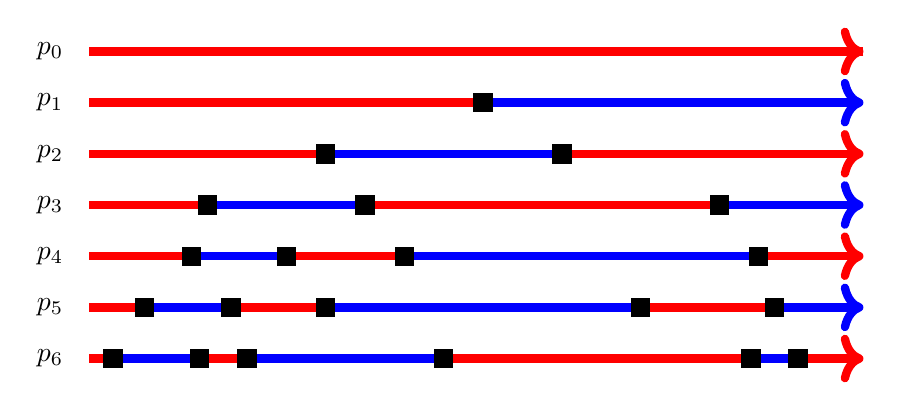
\begin{tikzpicture}[line width=3pt]
 		% Define the list of lists
 		\def\listOfLists{{},{5},{3,6},{1.5,3.5,8},{1.3,2.5,4,8.5},{0.7,1.8,3,7,8.7},{0.3,1.4,2,4.5,8.4,9}}
 		
 		% Define the colors for alternating connections
 		\definecolor{color1}{RGB}{0, 0, 255}
 		\definecolor{color2}{RGB}{255, 0, 0}
 		\colorlet{linecolor}{color1}
 		% Define the vertical spacing between levels
 		\def\verticalSpacing{-0.65}
 		
 		% Initialize the y-coordinate
 		\pgfmathsetmacro{\ycoord}{0}
 		
 		% Loop through the list of lists
 		\newcounter{arraycard}
 		\foreach \level [count=\i] in \listOfLists {
 			% Get the length of the current \level
 			\setcounter{arraycard}{0}%
 			% Draw nodes for each element in the sublist
 			\foreach \x [count=\j] in \level {
 				\pgfmathparse{\ycoord + (\i - 1) * \verticalSpacing}
 				
 				\node[mark=square, draw, fill=black, inner sep=2pt] (node\i\j) at ($(\x, \pgfmathresult)$) {};
 			}
 			
 			% Connect nodes on the same level with alternating colors
 			
 			\foreach \x [count=\j] in \level {
 				\let\ycoord\pgfmathresult
 				\ifodd\j
 				\colorlet{linecolor}{color2}
 				\else
 				\colorlet{linecolor}{color1}
 				\fi
 				\ifnum\j>1
 				\draw[linecolor] (node\i\j) -- (node\i\the\numexpr\j-1\relax);
 				\fi
 				\stepcounter{arraycard}%
 			}
 			% Use \levelLength to access the length of the \level
 			%\node[above right] at (node\i\the\value{arraycard}) {\the\value{arraycard}\ elements};
 			\pgfmathparse{int(\i-1)}
 			\node[draw=none] (node\i0) at ($(0, \ycoord + \i* \verticalSpacing - 1 * \verticalSpacing)$) {};
 			\node (name\i) at ($(node\i0)+(-0.5,0)$) {$p_\pgfmathresult$};
 			\pgfmathparse{int(\the\value{arraycard}+1)}
 			\node (node\i\pgfmathresult) at ($(10, \ycoord + \i* \verticalSpacing - 1 * \verticalSpacing)$) {};
 			\draw[color2] (node\i1) --($(0, \ycoord + \i* \verticalSpacing - 1 * \verticalSpacing)$);
 			
 			\ifodd\the\value{arraycard}
 			\colorlet{linecolor}{color1}
 			\else
 			\colorlet{linecolor}{color2}
 			\fi
 			\pgfmathparse{int(\the\value{arraycard}+1)}
 			\draw[linecolor,->] (node\i\the\value{arraycard}) -- (node\i\pgfmathresult);
 		}
 	\end{tikzpicture}
 	
 	\caption{
 		Visualizing zeros of the different levels of characteristic polynomials and their interlaced zeros. The lines represent the real $x$ axis, indicating where the value of the polynomial is {\color{red}positive (red)} or {\color{blue}negative (blue)} or zero ($\blacksquare$)
 	}\label{fig:charpoly-zero}
 \end{figure}
 
 This means that we can construct a hierarchy of the zeros of these polynomials and use information about all of their signs to tell how many zeros fall below a given value. \autoref{fig:charpoly-zero} nicely illustrates this structure and leads us to a couple of observations. Let's denote the number of sign flips in the sequence of polynomilas (evaluated at a certain $x$) $p_n(x), p_{n-1}(x), \dots, p_1(x), p_0(x)$ by $s(x)$ . 
 \begin{enumerate}
 	\item At the negative side as $x \to -\infty$, we see that since the leading term of the $j^{\mathrm{th}}$ polynomial is $\left(-1\right)^j x_j$, therefore $p_j \to \infty$, and hence the sign will be positive for all polynomials at a sufficiently low $x$, which results in $s(x)\to0$. On the flip side, for sufficiently large $x$ however $s(x)$ as the signs will alternate due to the $\left(-1\right)^j$ term.
 	\item Coming from negative $x$ values, between two eigenvalues, i.e. zeros of $p_n$, the number sign flips cannot change. This is due to the propery of interlaced zeros: if $p_j(x)$ flips in sign, then $p_{j+1}$ must have had a zero before that which flipped it, i.e. it will have the same sign as $p_j(x)$.
 	\item This leads to the last conclusion: $p_n$ introduces sign flips (because there is no $p_{n+1}$) at each of it's zeros, which are the eigenvalues.
 \end{enumerate}
 
 Thereby we can conclude that $s(x)$ describes the number of eigenvalues of $T$, which are smaller than $x$. This leads to an algorithm based on the idea of the bisection method to find $\lambda_k = \inf_{x} \left\lbrace x | s(x)=k\right\rbrace$, which will correspond to the $k^{\mathrm{th}}$ eigenvalue of $T_j$.
 
 \begin{algorithm2e}[ht]
 	
 	\SetKwInOut{Input}{input}
 	\SetKwInOut{Output}{output}
 	\SetKw{Init}{init}{}{}
 	\SetAlgoLined
 	\Input{Real symmetric tridiagonal matrix $T_j\in\mathbb{R}^{j\times j}$, given by diagonals $\mathbf{\alpha},\mathbf{\beta}$, $k$ index ($k\leq j$)}
 	\Output{$\lambda_k$ eigenvalue of $T_j$}
 	\Init{$\beta_0 = \beta_{j} = 0$}\\
 	\tcc{Lower and upper bounds of the eigenvalues using the Gershgorin circle theorem}
 	$R_i = \left|\beta{i-1}\right|+\left|\beta{i}\right|$ \textbf{for} $i=1,2,\dots,j$\\
 	$a = \min_{1\leq i \leq j}{\left(\alpha_{i}-R_i\right)}$\\
 	$b = \max_{1\leq i \leq j}{\left(\alpha_{i}+R_i\right)}$\\
 	\tcc{Bisection method}
 	\While{$\frac{b-a}{b} > \kappa$}{
 		$c = \frac{a+b}{2}$\\
 		\tcc{Using \autoref{alg:char-poly-eval} to evaluate $s(c)$ in $\mathcal{O}(j)$}
 		\uIf{$s(c, \alpha, \beta) < k$}{$a=c$}
 		\Else{$b=c$}
 	}
 	$\lambda_k = \frac{a+b}{2}$
 	\caption{Finding the $k^{\mathrm{th}}$ eigenvalue of the tridiagonal matrix $T_j$ with $\kappa/2$ precision}\label{alg:eigfind-Tj}
 \end{algorithm2e}
 
Note that if a $\beta_l$ is zero, that will break up the matrix into two blocks. This leads to the natural conclusion that in case of zero betas we can just recursively apply the algorithm. In a slightly more sophisticated fashion we could generalize the algorithm \autoref{alg:eigfind-Tj} so that it searches the blocks separately until out of $b$ blocks you find the one the $k^{\mathrm{th}}$ eigenvalue of the whole matrix, i.e. the $b$ blocks collectively have $k-1$ less eigenvalues smaller.

\subsection{Stability of the eigenvalue algorithm}

If we apply the above algorithm for finding eigenvalue we will soon notice a limitation of the algorithm for larger matrices: it simply fails to work for sizes from $\sim 800$ and up. The reason has to do with the evaluation of the sequence of polynomials which results in a faulty $s(x)$. This root cause, as noted by \textcite{stable_polys_Barth_Martin_Wilkinson_1967} is that during the evaluation of the polynomial sequence floating point number overflow happens. To prevent this a more stable sequence is suggested by \autocite{stable_polys_Barth_Martin_Wilkinson_1967}, namely one that keeps track of the ratio of the polynomials so that 
\begin{equation}
	q_{i} = \frac{p_i(x)}{p_{i-1}(x)} \quad \mathrm{for}\, i = 1, 2, \dots n.
\end{equation}
Thereby the recursion transforms into 
\begin{align}
	q_{0}(x) &= \alpha_1 - x,\\
	q_{i}(x) &= \alpha_i - x - \frac{\beta_{i}^2}{q_{i-1}(x)}.
\end{align}

This seems to aleviate the problems one might face in the next section.

Here as a test case two randomly generated tridiagonal symmetric matrices are used to test the algorithm in \autoref{fig:eig-stability}, which suggests that the stabilized version works well.
\begin{figure}[h!]
	\centering
	\begin{subfigure}{0.35\textheight}
		\centering
		\includegraphics[width=\textwidth]{../plots/eig_rand_test_k25_s0.pdf}
		\subcaption{Random tridiagonal matrix with $n=25$, \textbf{unstable} eigenvalue algorithm}
	\end{subfigure}
	\begin{subfigure}{0.35\textheight}
	\centering
	\includegraphics[width=\textwidth]{../plots/eig_rand_test_k800_s0.pdf}
	\subcaption{Random tridiagonal matrix with $n=800$, \textbf{unstable} eigenvalue algorithm}
	\end{subfigure}
	
	\begin{subfigure}{0.35\textheight}
	\centering
	\includegraphics[width=\textwidth]{../plots/eig_rand_test_k25_s1.pdf}
	\subcaption{Random tridiagonal matrix with $n=25$, \textbf{stable} eigenvalue algorithm}
	\end{subfigure}
	\begin{subfigure}{0.35\textheight}
	\centering
	\includegraphics[width=\textwidth]{../plots/eig_rand_test_k800_s1.pdf}
	\subcaption{Random tridiagonal matrix with $n=800$, \textbf{stable} eigenvalue algorithm}
	\end{subfigure}
	
	\caption{Testing the \textbf{stable} and \textbf{unstable} eigenvalue finding algorithms for two random suitable matrices. Apart from the eigenvalues $s(x)$ is also compared to the matlab \texttt{eig} function's results.}\label{fig:eig-stability}
\end{figure}

\subsubsection*{Finding mutliple eigenvalues at the same time}

To be more optimal at recycling information, one could develop a recursive algorithm for calculating a set of desired eigenvalues, where each evaluation of $s(x)$ is used to its maximal potential. \autoref{alg:eigfind-Tj-recursive} descirbes such an algorithm. Here let us denote the set of whole numbers between $a$ and $b$ ($a<b$) with 
\begin{equation*}
	\Upsilon(a,b) = \left\lbrace a, a+1, a+2, \dots b-1, b\right\rbrace
\end{equation*}

\begin{algorithm2e}[h!]
	
	\SetKwInOut{Input}{input}
	\SetKwInOut{Output}{output}
	\SetKw{Init}{init}{}{}
	\SetAlgoLined
	\Input{Real symmetric tridiagonal matrix $T_j\in\mathbb{R}^{j\times j}$, given by diagonals $\mathbf{\alpha},\mathbf{\beta}$, $K$ set of integer indicies}
	\Output{$\left[\lambda_k\right]_{k \in K}$ eigenvalues of $T_j$, trying to preserve multiplicity}
	\Init{$\beta_0 = \beta_{j} = 0$}\\
	\tcc{Lower and upper bounds of the eigenvalues using the Gershgorin circle theorem}
	$R_i = \left|\beta{i-1}\right|+\left|\beta{i}\right|$ \textbf{for} $i=1,2,\dots,j$\\
	$a = \min_{1\leq i \leq j}{\left(\alpha_{i}-R_i\right)}$\\
	$b = \max_{1\leq i \leq j}{\left(\alpha_{i}+R_i\right)}$\\
	\Return{\texttt{SetBisect}$\left(K, a, b,\alpha, \beta\right)$}\\
	\tcc{Recursive bisection method}
	\SetKwFunction{FMain}{SetBisect}
	\SetKwProg{Fn}{Function}{:}{}
	\Fn{\FMain{$K, a, b, \alpha, \beta$}}{
		\uIf{$|K|=0$}{\Return{$[\quad]$\tcp{No eigenvalues in this interval to be found}}}
		\uElseIf{$\frac{b-a}{b} < 2\epsilon$}{
			\tcp{The eigenvalues could not be resolved any further}
			\Return{$\underbrace{\left[\frac{a+b}{2},\,\frac{a+b}{2},\,\dots,\frac{a+b}{2}\right]}_{\left|K\right| \,\mathrm{ elements}}$}
		}
		\uElseIf{$\frac{b-a}{b} > \kappa$ \textbf{or} $|K| > 1$}{
			$c = \frac{a+b}{2}$\\
			\tcc{Using \autoref{alg:char-poly-eval} to evaluate $s(c)$ in $\mathcal{O}(j)$. Values are cached in reality}
			\Return{\texttt{SetBisect}$\left(K \cap \Upsilon\left(s(a),s(c)\right),a,c,\textsc{} \alpha, \beta\right)\,$ $\cup\footnotemark\,$ \texttt{SetBisect}$\left(K \cap \Upsilon\left(s(c),s(b)\right),c, b, \alpha, \beta\right)$\tcp{Recursion}}
		}
		\Else{\Return{$\left[\frac{a+b}{2}\right]$}\tcp{Eigenvalue resolved with $\frac{\kappa}{2}$ precision in this interval}}
	}
	\textbf{End Function}
	\caption{Finding a set $K$ eigenvalues of the tridiagonal matrix $T_j$ with $\kappa/2$ precision}\label{alg:eigfind-Tj-recursive}
\end{algorithm2e}
\footnotetext{Interpret $\cup$ as concatenation for arrays}

\FloatBarrier
\section{Atomic Force Microscopy}
\subsection{Background}
\begin{figure}[ht]
	\includegraphics[width=.5\linewidth,height=4.5cm]{../afm_tip.jpg}
	\includegraphics[width=.5\linewidth,height=4.5cm]{../afm_principle.png}
\end{figure}
Atomic force microscopy (AFM) is a microscopy technique that works on the same length scales a
scanning tunneling microscopy (STM), but does not need its subject to be electrically conductive.
The driving transmitted of information is not tunneling electons, but various atomic forces. This
makes AFM better suited to study proteins, blood cells, etc. than STM.\\


The basic priciple is that a cantilever with a small tip at its free end is brought close to, or in contact
with a material or material surface. A concentrated light beam is bounced off of the cantilever and
captured on a light sensitive receiver. Then the movement of the cantilever due to atomic forces can
be recorded and information on the sample can be deduced.
AFM comes in three modes: contact mode, tapping mode and non-contact mode.For this homework,
we are only interested in the non-contact mode.\\


In non-contact atomic force microscopy the cantilever tip does not come in contact with the sample
surface, but rather sits at some distance, where chosen non-contact forces are strongest. For instance
the van der Waals forces are strongest from 1 nm to 10 nm above the surface. The cantilever is oscillated
at one of its resonant frequencies (frequency modulation) or just above one (amplitude modulation).
The long-range forces above the surface decrease the resonance frequency of the cantilever. By moving
the tip closer and further this decrease can be counteracted. As such, a constant oscillation (in
amplitude or frequency) is created, which can be used to measure the distance to the sample. Since
this mode of AFM operation does not actually contact the sample, it is much more suited for the
observation of delicate systems.\\


Additionally, the cantilever oscillation frequencies and modes can provide insight into the types of
forces acting on the AFM system and even on the indiviual atoms that the sample is made up of.
It should be clear to you from these considerations that a rigorous modal analysis of the AFM cantilever
is absolutely vital. This is what we will do in this final part of the assignment.
\subsection{Modal analysis using the finite element method}
In a modal analysis the typical assumption is that of undamped harmonic motion without driving
forces. Whenever the given volume is discretized to a mesh and a choice of basis functions is made
(taking boundary conditions into account) this leads to a system

\begin{equation}\label{eq:gen-eig}
	(K - \omega^2 M)\delta \mathbf{u} = 0
\end{equation}
with
$$\delta \mathbf{u}=\begin{pmatrix}
	\delta \mathbf{u}_x\\
	\delta \mathbf{u}_y\\
	\delta \mathbf{u}_z
\end{pmatrix}\footnotemark$$
\footnotetext{One can see from the roughly similar $3\times 3$ blocks in the matrices that result from such an ordering of the displacement vector.}
a vector of displacements. Such a problem is called a generalized eigenvalue problem. The matrix $K$
is called the stiffness matrix, and the matrix $M$ is called the mass matrix. Note that each node of the
given grid produces three degrees of freedom (dof). Elements in the stiffness matrix correspond to the
stiffness at dof-dof interactions (e.g. the xy-stiffness at a given node), and the elements of the mass
matrix correspond to the masses at the corresponding dof-dof interactions. 
It stands to reason therefore that $M$ and $K$ will be symmetric real (and in most cases positive definite).

Before the solving the system, boundary conditions have to be applied. In this particular case only homogeneous Dirichlet boundary conditions have to be applied, which mean that the components of $\delta \textbf{u}$ corresponding to certain nodes in the mesh have to be set to zero: these are the fixed ends of the cantilever. Since we are talking about the components being set to zero, this wont affect the right hand side of \autoref{eq:gen-eig}, so we will assume moving forward that the rows and columns corresponding to these elements have been removed already.

\subsection{Transformation into regular eigenvalue problem}
Since the matrices $M, K$ are symmetric, we can employ the singular value decomposition to transform the problem into the standard eigenvalue problem. Let's assume that we perform the singular value decompositon on $M$ as follows
\begin{equation}
	M = U S V^\ast = U S U^\ast
\end{equation}
where in our particular case since all of the singular values are non-zero, $S$ will be a full diagonal matrix, while $U=V$ orthonormal/unitary.
Since the singular values are all non-negative by definition we can construct the cholesky factorization as 
\begin{equation}
	M = U S ^{\frac{1}{2}} \left(U S ^{\frac{1}{2}}\right)^ast,
\end{equation}
where $S ^{\frac{1}{2}}$ is simply the elementwise square root of the diagonal matrix. Armed with this we can reformulate the problem in \autoref{eq:gen-eig} as 
\begin{equation}\label{eq:stand-eig}
	U S^{\frac{1}{2}} \bigl( \underbrace{S^{-\frac{1}{2}} U^\ast K U S^{-\frac{1}{2}}}_{A} - \omega^2 I\bigr)S^{\frac{1}{2}} U^\ast \delta \mathbf{u} = 0 
\end{equation}
Therefore we see that \autoref{eq:stand-eig} is already a standard eigenvalue problem for a symmetric matrix.

\subsection{Numerical approximation of the eigenvalues}
Now we can use the Lanczos method (in this case \texttt{Lanczos2} or \texttt{Lanczos3}) to transform $A$ into tridiagonal form, where the eigenvalues can be estimated using the methods described in \autoref{sec:eig-tri}, e.g. \autoref{alg:eigfind-Tj} with the stabilized characteristic polynomial evaluation. Such an algorithm is demonstrated using in \autoref{code:solve-afm}, where we check whether this method preserves and correctly estimates the eigenvalues of the matrix. 

We can see in \autoref{fig:afm-eig} that the eigenvalues of \autoref{eq:gen-eig} and \autoref{eq:stand-eig} perfectly cover eachother, therefore our manipulation of the system with the SVD has not distorted the results. Gurthermore we can see thet with only 300 ($k_{\mathrm{max}}= 300$) Ritz values the Lanczos algorithm is doing a pretty good job of approximating the spectrum. The stabilized \autoref{alg:eigfind-Tj} (with $k=1,2,3,4,5,\dots$ as the lowest values' indicies) perfectly finds the lowest eigenvalues of the system as one can see.
\begin{figure}[h!]
	\centering
	\resizebox{0.8\textwidth}{!}{
		\input{../plots/afm_eigs.tex}}
	\caption{The various eigenvalues $\left(\omega_i^2\right)$ of the generalized eigenvalue problem in \autoref{eq:gen-eig} (${\color{blue}-}$), and of $A$ (${\color{red}-}$) from \autoref{eq:stand-eig} obtained using \texttt{Matlab}'s built in \texttt{eig} function. The eigenvalues/Ritz values of $T_k$ (${\color{yellow}\times}$) from \texttt{eig} and our custom \texttt{eigval\_k} (${\color{purple}\times}$) from \autoref{alg:eigfind-Tj} (with which only the first few are calculated) are marked with $\times$'s. Their $x$ coordinates are distorted so as to distribute them over the same length as the explicitly calculates values }\label{fig:afm-eig}
\end{figure}

The calculated first 5 eigenfrequencies of the system are compared in \autoref{table:eig-calc-300}. We can see that while the respective techniques do give similar results before and after the Lanczos decomposition, however it is impossible to require of the Ritz values to converge faster to the lowest eigenvalues, as they are trying to cover the entire spectrum most optimally, and these values are outliers. A higher number of iteration steps ($k_{\mathrm{max}}$) would of course lead to better estimations but increase computational costs.

\begin{table}[h!]
	\centering
	\caption{Eigenvalues calculated with various methods (For the Lanczos various sizes are used}\label{table:eig-calc-300}
	\begin{tabular}{r|c|c|c|c|c|c}
		method & $k_{\mathrm{max}}$ & $\omega_1$& $\omega_2$& $\omega_3$& $\omega_4$& $\omega_5$ \\\hline\hline
		\texttt{eig(K,M)} &-&  1.0020864e+02 & 5.2977376e+02 & 6.7732332e+02 & 1.1282088e+03 & 1.6398795e+03\\\hline
		\texttt{eig(A)} &-& 1.0020864e+02 & 5.2977376e+02 & 6.7732332e+02 & 1.1282088e+03 & 1.6398795e+03\\\hline\hline
		\texttt{eig(T\_k)} &300& 2.6346086e+03 & 8.8949675e+03 & 1.4536307e+04 & 2.0342715e+04 & 2.6965513e+04 \\\hline
		\texttt{eigval\_k(A)} &300& 2.6346086e+03 & 8.8949675e+03 & 1.4536307e+04 & 2.0342715e+04 & 2.6965513e+04\\\hline\hline
		\texttt{eigval\_k(A)} &900& 7.4794369e+02 & 2.5283561e+03 & 3.5036295e+03 & 5.9547354e+03 & 7.5757296e+03\\\hline\hline
		\texttt{eigval\_k(A)} &1500& 5.3315103e+02 & 1.6230993e+03 & 2.5812411e+03 & 3.0990669e+03 & 4.3763682e+03\\\hline\hline
		\texttt{eigval\_k(A)} &2424\footnote{Max unconstrained dimensions of the system}& 1.0020864e+02 & 5.2977376e+02 & 6.7732332e+02 & 1.1282088e+03 & 1.6398795e+03\\\hline\hline
	\end{tabular}
	 
	 
	
	
\end{table}
 
\FloatBarrier

\begin{code}
	\inputminted[mathescape,linenos,frame=lines,firstline=7,lastline=30]{matlab}{../tests/solve_afm.m}
	\captionof{listing}{\texttt{solve\_afm.m}}
	\label{code:solve-afm}
\end{code}
	
\subsection{Visualization of the modes}

To calculate the eigenvectors, we can rely on the built in \texttt{null} function of \texttt{Matlab}, which calculates a basis of the nullspace $\mathcal{N}(A)$ of a given matrix. However in order to make this work the Lanczos algorithm must be run for the entire matrix, lest we will not be able to get a null-vector. In desperate cases other techniques (such as fixing a value in $\delta\textbf{u}$, and calculating the rest of the values according to the resulting inhomogeneus linear equation). Using basic linear algebra and leveraging the unitary property of $U$, we know that for a calculated eigenvalue $\omega_i^2$ we can get the eigenvector by  
\begin{equation}
	w_i \in \mathcal{N}(A-\omega_i^2 I), \quad \delta \textbf{u}_i = U S^{-\frac{1}{2}} w_i  \leftrightarrow K \delta \textbf{u}_i = \omega_i^2 M \delta \textbf{u}_i. 
\end{equation}
This gives us a convenient way of calculating the eigenvectors.

The calculated displacement modes are visualized in \autoref{fig:eig-modes} together with the mesh itself. It is important to note that the most energy is usually stored in the lowest eigenfrequency of such a system, so mode 1 is the most relevant. 
We can observe that the higher frequencies correspond to more and more complicated vibration shapes. Mode 1 is the most straighforward simple bobbing of the tip, which is most important and imaginable for us.

\begin{figure}[h!]
	\centering
	\begin{subfigure}{0.35\textheight}
		\centering
		\includegraphics[width=0.8\textwidth]{../plots/afm_mesh.pdf}
	\end{subfigure}
	\begin{subfigure}{0.35\textheight}
		\centering
		\includegraphics[width=0.9\textwidth]{../plots/afm_mesh_mode1.pdf}
	\end{subfigure}
	
	\begin{subfigure}{0.35\textheight}
		\centering
		\includegraphics[width=0.9\textwidth]{../plots/afm_mesh_mode2.pdf}
	\end{subfigure}\begin{subfigure}{0.35\textheight}
	\centering
	\includegraphics[width=0.9\textwidth]{../plots/afm_mesh_mode3.pdf}
	\end{subfigure}
	
	\begin{subfigure}{0.35\textheight}
		\centering
		\includegraphics[width=\textwidth]{../plots/afm_mesh_mode4.pdf}
	\end{subfigure}\begin{subfigure}{0.35\textheight}
	\centering
	\includegraphics[width=0.9\textwidth]{../plots/afm_mesh_mode5.pdf}
	\end{subfigure}
	
	\caption{The mesh and the dominant (smallest $\omega$) eigenmodes of the cantilever model.}\label{fig:eig-modes}
\end{figure}

\FloatBarrier
\newpage
\printbibliography
\end{document}